\documentclass[10pt]{article}

\usepackage{amsmath}% http://ctan.org/pkg/amsmath
\usepackage{amsthm}
\usepackage{todonotes}
\usepackage[margin=1in]{geometry}
\usepackage{algorithm}
\usepackage{url}
\usepackage[noend]{algpseudocode}
\usepackage{mdframed}
\usepackage{tikz}
\usepackage{enumerate}
\usetikzlibrary{matrix,shapes,arrows,positioning,chains, calc}

%% defining new theorem environment for definition
\newtheorem{defn}{\textbf{Definition}}
\newtheorem{thm}{\textbf{Theorem}}
\newtheorem{cor}{\textbf{Corollary}}
\newtheorem{lemma}{\textbf{Lemma}}

\renewcommand{\algorithmicrequire}{\textbf{Input:}}
\renewcommand{\algorithmicensure}{\textbf{Output:}}

\begin{document}
\title{IP-to-NDN Application-Layer Gateway Middleware}
\author{Christopher A. Wood \\ {\tt woodc1@uci.edu}}
\date{\today}
%\thanks{TODO}
\maketitle

%%%%%%%%%%%%%%%%%%%%%
%%% MAIN CONTENT
%%%%%%%%%%%%%%%%%%%%%

\section{Introduction}
Today's Internet architecture is largely inspired by traditional communication-based switching networks. Consequently, it has been retrofitted with a variety of transport and application layer protocols and middleware to support a growing set of consumer applications. Of particular importance are content distribution applications, such as media streaming services similar (e.g., Netflix), which leverage the underlying communication-based network as a distribution network and continue to consume vital networking resources at a rapidly increasing pace. Information-centric networks (ICNs) are a new class of network architectures that aim to address this increasingly popular type of network traffic by decoupling data from its source and shifting the emphasis of addressable content from hosts and interfaces to content \cite{}. By directly addressing content instead of hosts, content dissemination and security can be decoupled from the source and distributed throughout the network. 

Currently, several information-centric networking proposals are being explored as alternative designs to today's public Internet, with Named Data Networking (NDN) \cite{NDNtech} being one of the more promising designs. While promising, its design still an area of active research. As a replacement for IP-based networks, the complete adoption of any one of these designs will realistically be done in by slow and continual integration and replacement of IP-based networking resources with ICN-based resources. Currently, however, there is no engineering plan to support the IP-to-ICN integration. 

Consequently, the primary objective of this project is to aid the integration of future content-centric networking resources into the existing IP-centric Internet by providing an application-layer gateway between IP and NDN resources. Application-layer traffic corresponding to protocols such as HTTP, FTP, SMTP, IMAP, etc. will be translated by middleware running in such gateways to correctly interface with the NDN resources. 

\section{Overview}
The NDN architecture enables relevant content to be pushed and stored throughout the network to minimize overall bandwidth consumption. Network caches and addressable content, rather than addressable hosts or interfaces, promote reduced network congestion and latency by keeping content closer to its intended recipients. The process by which content is requested is through the issuance of an \emph{interest}. Routers that have cached content matching the interest name, or producers who advertise that they provide content matching the name, may respond with the corresponding (cryptogrpahically signed) piece of content. As such, content flows through the same network path from which the interest originated. 

This type of content retrieval strategy is fundamentally distinct from IP-based content distribution. Therefore, this NDN gateway is a server and middleware software stack designed to support the translation from IP-based to NDN-based communication and messages. For example, HTTP GET requests would be intercepted and translated into an interest for the same piece of content. The procedure for doing this translation 

% \begin{figure}
% \begin{center}
% 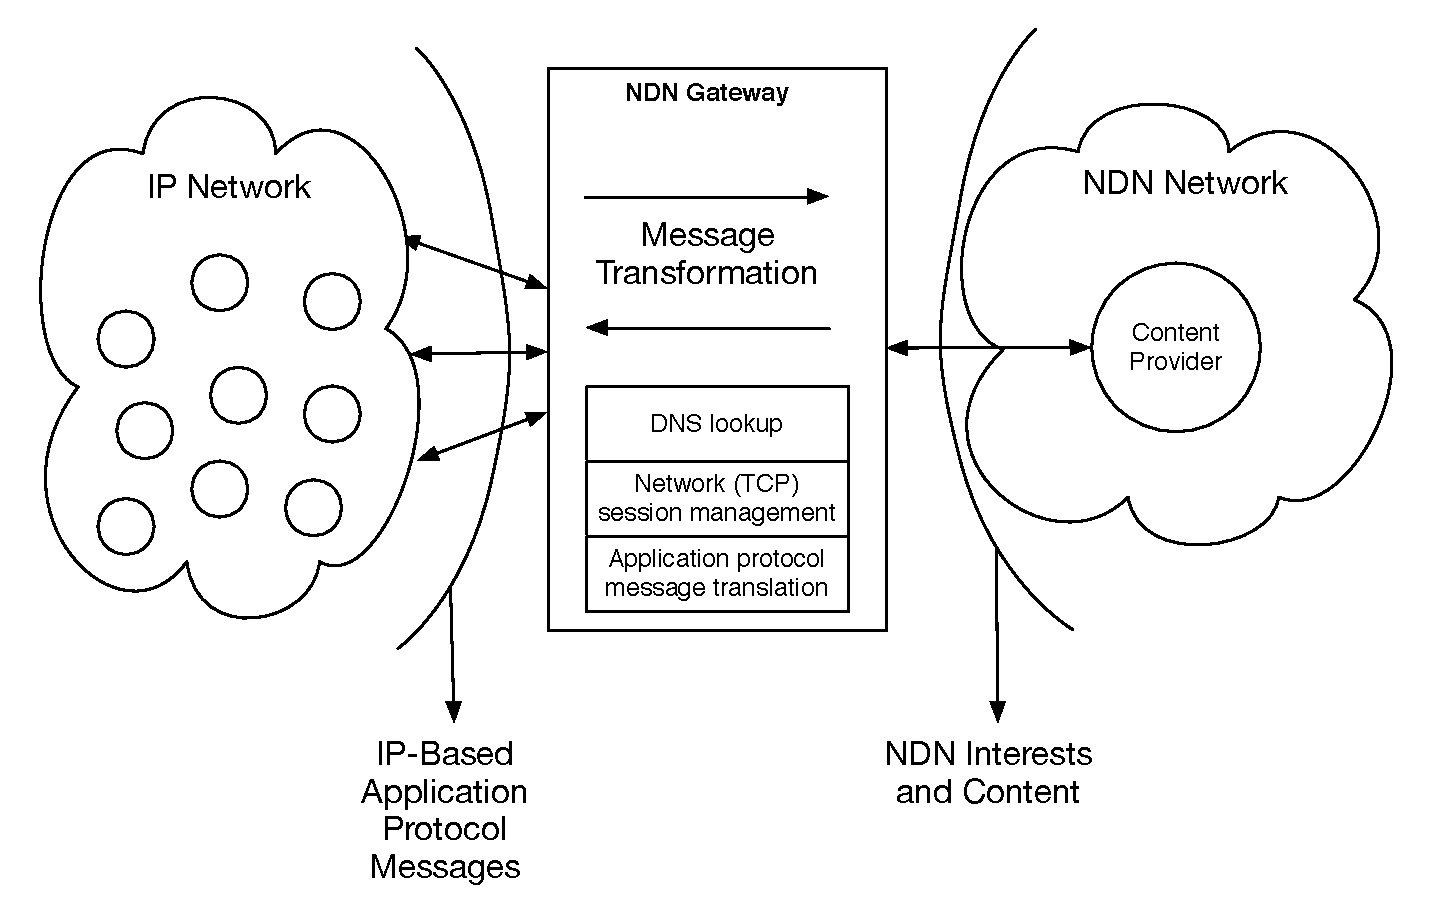
\includegraphics[scale=0.5]{images/gateway_highlevel.pdf}
% \end{center}
% \end{figure}

\section{Implementation Highlights and Milestones}
The implementation of this project will be done using both C/C++ and Java libraries, and will rely on the open-source CCNx \cite{ccnx} library for development. Architecturally, the middleware will be partitioned among a Java-based front-end for intercepting all IP-based traffic and performing application-layer protocol translation, and a C-based backend utilizing the CCNx library to interface with NDN network resources, and a web interface that can be used to configure the gateway. Consequently, the deliverables for this project is a software design and architecture document, application gateway source code, and web interface (for gateway configuration). A preliminary timeline for the major milestones of this project is given below.

\begin{enumerate}[{\bf Week} 1:]
	\setcounter{enumi}{2}
	\item Project proposal and preliminary project experiments
	\item Front-end skeleton, API design, and application-layer protocol listeners
	\item Back-end skeleton, design, and NDNx integration
	\item Java JNI integration and application-wide integration testing
	\item Middleware DNS lookup
	\item Middleware session management
	\item Middleware application layer translation
	\item Elementary web interface and finalize project experiments
	\item Conduct experiments and draft final report 
\end{enumerate}

%%%%%%%%%%%%%%%%%%%%%
%%% END MAIN CONTENT
%%%%%%%%%%%%%%%%%%%%%

%%% BIBLIOGRAPHY
\begin{thebibliography}{[MT1]}

\bibitem{NDNtech} Lixia Zhang, Deborah Estrin, Jeffrey Burke, Van Jacobson, James D. Thornton, Diana K. Smetters, Beichuan Zhang, Gene Tsudik, kc claffy, Dmitri Krioukov, Dan Massey, Christos Papadopoulos, Tarek Abdelzaher, Lan Wang, Patrick Crowley, and Edmund Yeh. Named Data Networking (NDN) Project. PARC Tech Report 2010-003, NDN-0001 (2010).

\bibitem{ccnx} Content Centric Networking (CCNx) - Project CCNx. Available online at: \url{https://github.com/ProjectCCNx/ccnx}. Last accessed: 4/2/14.

\end{thebibliography}

\end{document}
